\documentclass[11pt,a4paper]{article}
\usepackage[utf8]{inputenc}
\usepackage[T1]{fontenc}
\usepackage{amsmath}
\usepackage{amsfonts}
\usepackage{amssymb}
\usepackage[left=3.0cm, right=3.0cm, top=3.0cm, bottom=3.0cm]{geometry}
\usepackage{xcolor}
\usepackage{graphicx}
\usepackage{caption}
\usepackage{subcaption}

% include code listings
\usepackage{listings}

% Defining colors for syntax highlighting
\definecolor{codegreen}{rgb}{0,0.6,0}
\definecolor{codegray}{rgb}{0.5,0.5,0.5}
\definecolor{codepurple}{rgb}{0.58,0,0.82}
\definecolor{backcolour}{rgb}{0.95,0.95,0.92}

\lstdefinestyle{mystyle}{
	backgroundcolor=\color{backcolour},   
	commentstyle=\color{codegreen},
	keywordstyle=\color{magenta},
	numberstyle=\tiny\color{codegray},
	stringstyle=\color{codepurple},
	basicstyle=\ttfamily\scriptsize,
	breakatwhitespace=false,         
	breaklines=true,                 
	captionpos=b,                    
	keepspaces=true,                 
	numbers=left,                    
	numbersep=5pt,                  
	showspaces=false,                
	showstringspaces=false,
	showtabs=false,                  
	tabsize=2
}

\lstset{style=mystyle}
\captionsetup[lstlisting]{font={scriptsize}}

% header and footer
\usepackage{fancyhdr}
\pagestyle{fancy}
\fancyhf{}
\lhead{Michele Guadagnini}
\rhead{\today}
\lfoot{Panoramic Image Construction - Computer Vision 2021}
\rfoot{Page \thepage}

\author{Michele Guadagnini - ID 1230663}
\title{\textbf{Computer Vision 2021 - Final Project: \\ \textit{Panoramic Image Construction}}}
\date{\today}


\begin{document}
\maketitle

\vspace{20pt}
\begin{abstract}
	The goal of this project is to construct a panoramic image starting from a sequence of images. 
	The procedure adopted starts from projecting the pictures into a cylindrical surface; in this way the transformations between adjacent images consists ideally in a simple translation.
	To compute the proper translation matrix the \textit{SIFT} features have been used together with the \textit{RANSAC} algorithm to select inlier keypoints.
	Some extra features are represented by the possibility to produce a panoramic image also in RGB colors and to apply a histogram equalization to the final image. \\
	The code has been developed in \textit{C++} language, making use of the \textit{OpenCV} library.
\end{abstract}

\section{Algorithm description} %Explain briefly the theory you have based your solution on.

The algorithm can be summarized as follows:

\begin{itemize}
	\item Firstly, the images are projected onto a cylindrical surface. This ideally allows to use a simple horizontal translation between the images to build up the panoramic images.  \\
	The projection requires to know the Field of View (\textbf{FoV}) used to capture the photos.
	
	\item The next step is to apply the Scale-Invariant Feature Transform (\textbf{SIFT}) algorithm to detect the local features in pictures. 
	Presented by Lowe in $2004$, it is useful in a lot of computer vision applications. Its greatest strength is that it allows to select the best scale for feature extraction. \\	
	In this work we use the local features extracted from the algorithm to match the consecutive images and find the translation that best merge them into one picture.
	
	\item The matches resulting from the SIFT features require to be filtered in order to keep only the useful ones. 
	A first refinement is done by selecting only the matches with distance less than their minimum distance multiplied by a certain coefficient to be defined by the user.
	Then the translation of an image with respect to the other is estimated by exploiting the \textbf{RANSAC} algorithm to select the inliers between the SIFT keypoints. Finally the translation is computed by calculating the average distance between inliers on both dimensions, obtaining the two coefficient needed to build the translation matrix.
	
	\item The last step is to merge all the projected images into one using the transformations computed above. To do this, the translations are combined together at each step.	
\end{itemize}

\section{Code Development} %Introduce strategies, tests, and report debugging problems, compilations options

The code development started by implementing the functions needed to complete the task inside a class, \textit{PanoramicUtils}. In Listing \ref{lst:header} it is reported the class definition, contained in the file \textit{panoramic\_utils.h}. 

\lstinputlisting[language=C++, firstnumber=19, linerange={19-58}, caption=PanoramicUtils class definition inside its header file., label=lst:header]{panoramic_utils.h}

The first function, the one performing the cylindrical projection, was already provided, but only to work with gray-scale images. To have the possibility to produce also color panoramics a new function has been created. This new function (\textit{cylindricalProjRGB}) do the same computations of the first one, but, instead of converting the image to gray-scale, it splits the 3 channels, applies the projection to each of them and finally restore the RGB image by merging the projected channels.

The other functions visible in Listing \ref{lst:header} follows the steps explained above in the algorithm description. It is worth to mention that the \textit{SIFT} descriptions has been computed by using the \textit{OpenCV} class \textbf{cv::SIFT} and the matches between them with the class \textbf{cv::BFMatcher}; they allowed to reduce the code needed for these tasks to few lines (see the implementation in \textit{panoramic\_utils.cpp} for details).

As suggested in the assignment, to apply the \textit{RANSAC} algorithm to select the best matches between keypoints the function \textbf{cv::findHomography} has been used and its argument \textit{mask} allowed to retrieve the inliers keypoints.

In the function \textit{build\_panoramic}, after merging all the images into one, it has been added a cropping of the panoramic image in order to remove the borders left by some small vertical translations. The code of this step is reported below in Listing \ref{lst:cropping}.

\lstinputlisting[language=C++, firstnumber=292, linerange={292-300}, caption=Code used to eliminate black borders from panoramic image., label=lst:cropping]{panoramic_utils.cpp}

The last function to be mentioned is the one that allows to perform the histogram equalization of the final image, \textit{intensity\_hist\_EQ}, which is reported in Listing \ref{lst:histeq}.
This function can equalize the histogram of a gray-scale image, but also a color image. To do this, the input image is firstly converted from \textbf{RGB} to \textbf{YCrCb} space, then equalization is applied to the \textbf{Y} (intensity) channel. By merging the channels again and converting back to RGB space, the equalized color image is obtained.

\lstinputlisting[language=C++, firstnumber=119, linerange={119-145}, caption=Function to perform histogram equalization to an image., label=lst:histeq]{panoramic_utils.cpp}

\subsection{Compilation and usage}

The program has been compiled with the following command:
\begin{lstlisting}[language=BASH,numbers=none]
	g++ -o panoramic Panoramic_main.cpp panoramic_utils.cpp `pkg-config --cflags --libs opencv`
\end{lstlisting}

Below it is reported a usage explanation of the executable:
\begin{lstlisting}[language=BASH,numbers=none] 
	./panoramic "images_path"  FoV  ratio  output_name  color_mode  equalization
\end{lstlisting}

The program also print a help message with usage instructions in case a wrong number of arguments have been passed.

\section{Results} %Present data and explain your results.

The first result presented is the panoramic image of the lab, reported also in the project description as an example. The image has been obtained also with colors, Figure \ref{fig:lab_g} and \ref{fig:lab_rgb}. Figure \ref{fig:lab_eq} instead reports the equalized panoramic view of the lab.

Also the panoramic images of the \textit{dolomites} and \textit{kitchen} datasets are reported in Figure \ref{fig:others}, both in gray-scale and colors.

\begin{figure}[h]
	\centering
	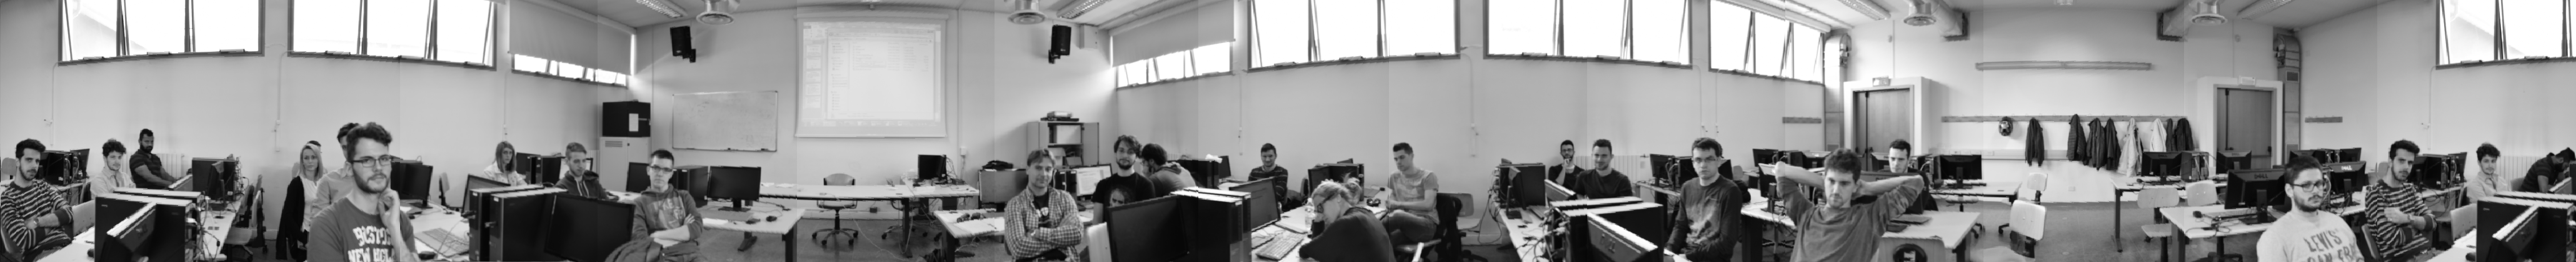
\includegraphics[width=1\linewidth]{lab_pan_gray.png}
	\caption{Laboratory panoramic view in gray-scale.}
	\label{fig:lab_g}
\end{figure}

\begin{figure}[h]
	\centering
	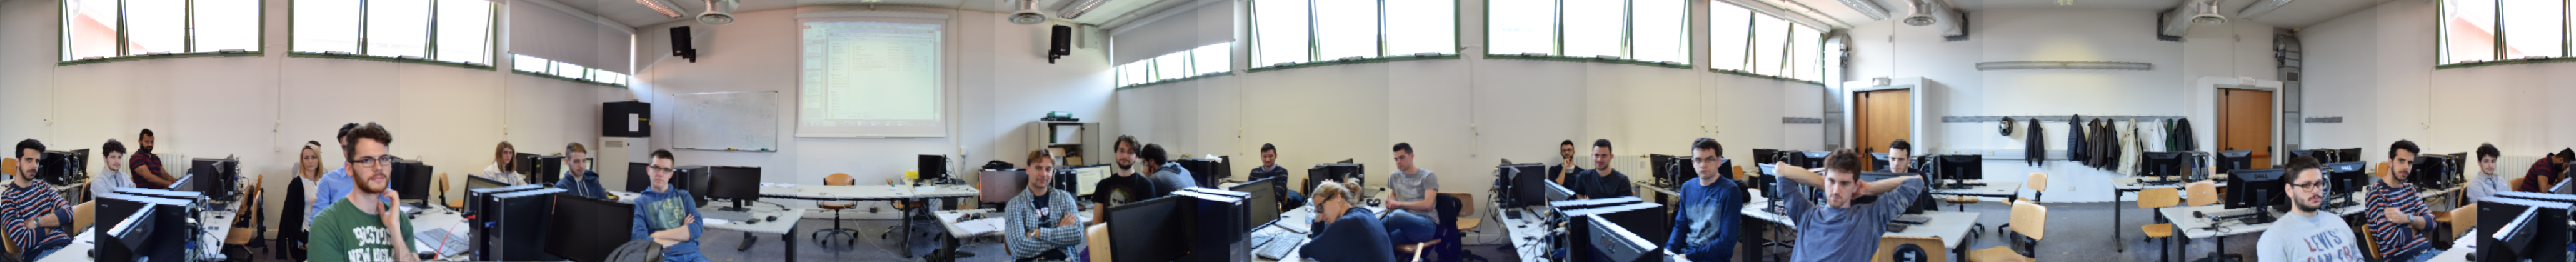
\includegraphics[width=1\linewidth]{lab_pan.png}
	\caption{Laboratory panoramic view with colors.}
	\label{fig:lab_rgb}
\end{figure}

\begin{figure}[h]
	\centering
	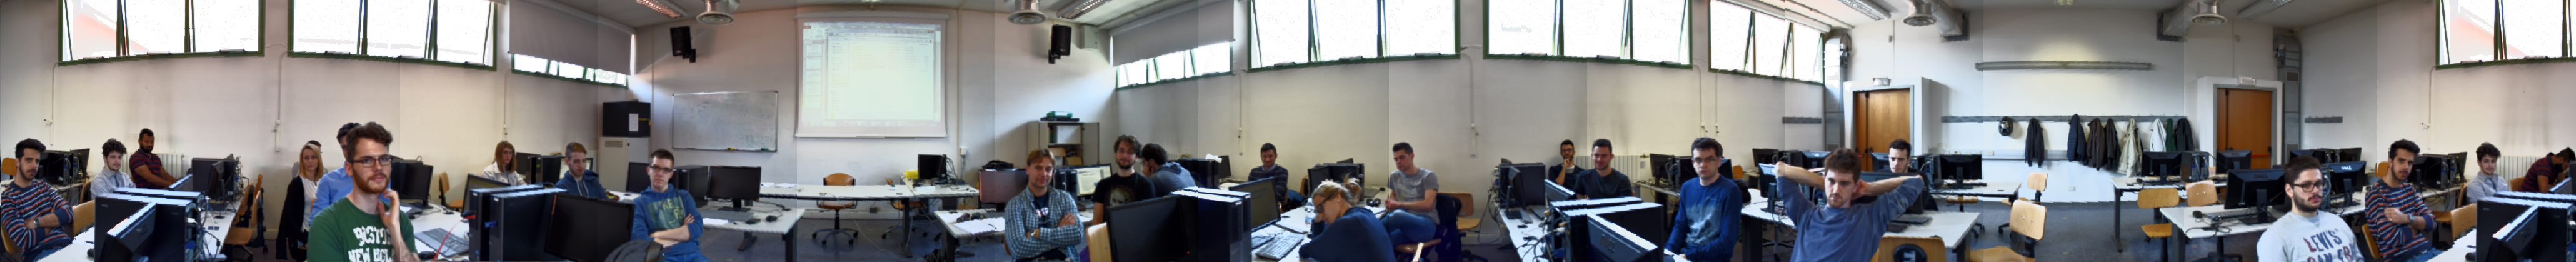
\includegraphics[width=1\linewidth]{lab_pan_eq.png}
	\caption{Laboratory panoramic view with colors after histogram equalization.}
	\label{fig:lab_eq}
\end{figure}

\begin{figure}[h]
	\centering
	\begin{subfigure}{1\textwidth}
		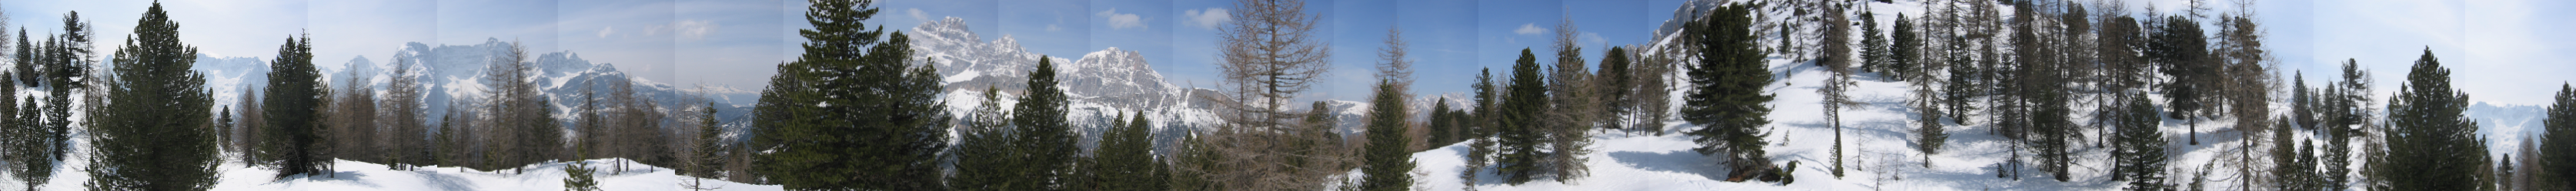
\includegraphics[width=1\linewidth]{dolomites_pan.png}
	\end{subfigure}
	\hfill
	\vspace{10pt}
	\begin{subfigure}{1\textwidth}
		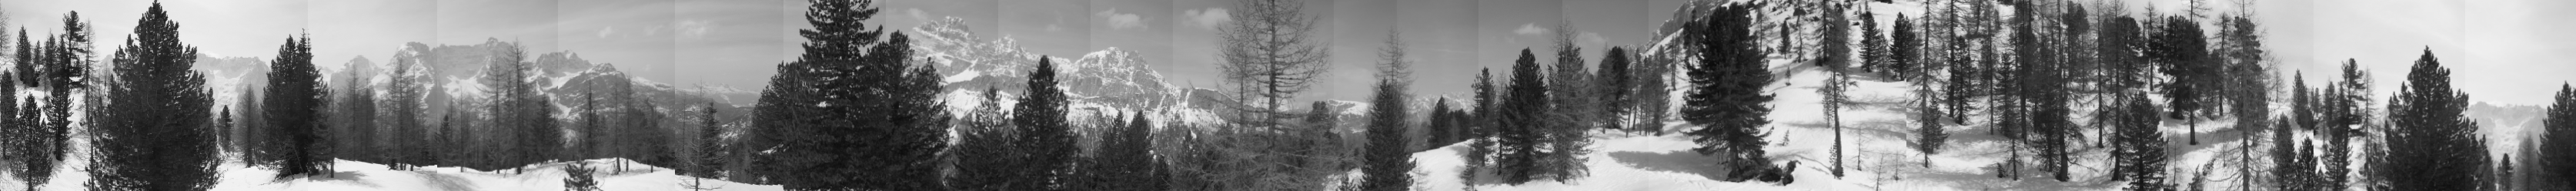
\includegraphics[width=1\linewidth]{dolomites_pan_gray.png}
	\end{subfigure}
	\hfill
	\vspace{10pt}
	\begin{subfigure}{1\textwidth}
		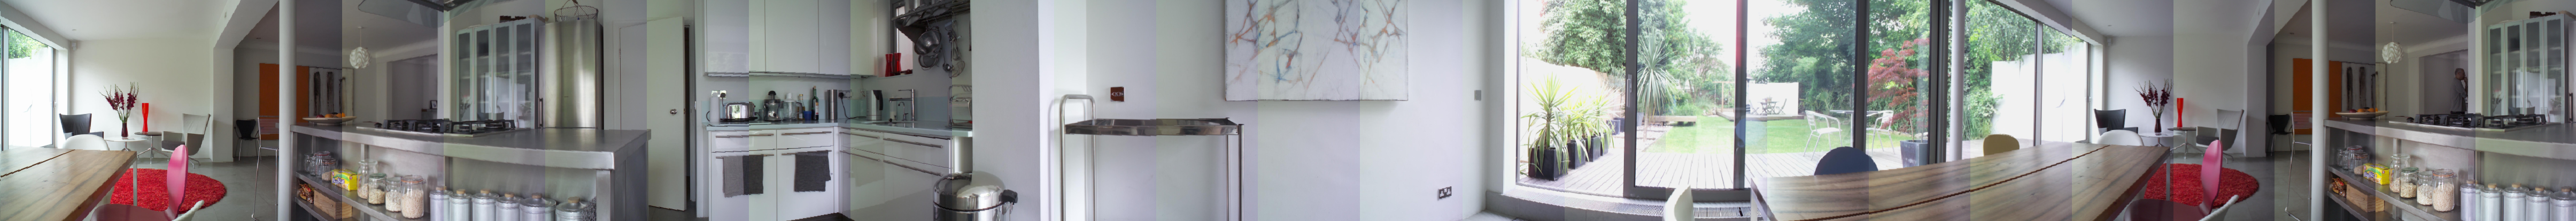
\includegraphics[width=1\linewidth]{kitchen_pan.png}
	\end{subfigure}%
    \hfill
    \vspace{10pt}
	\begin{subfigure}{1\textwidth}
		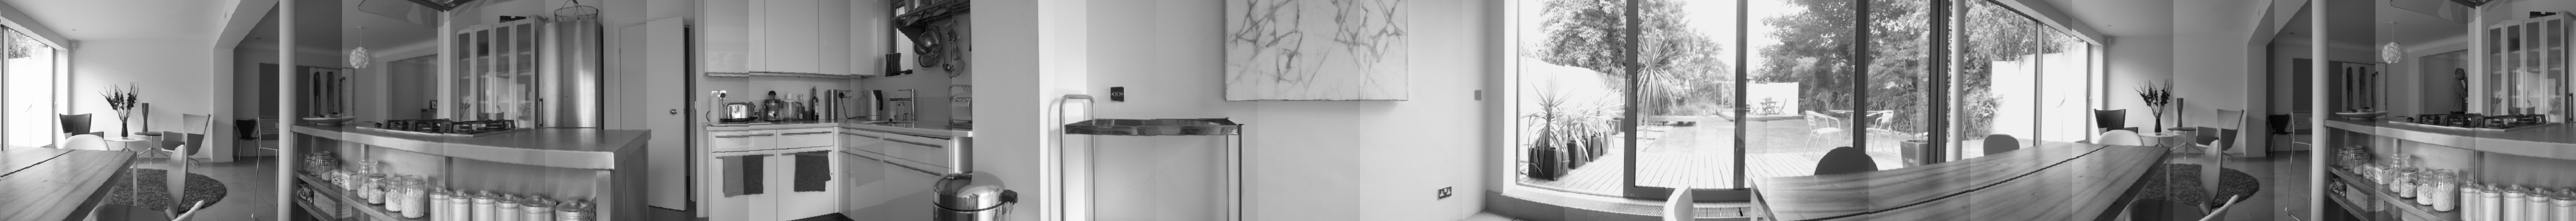
\includegraphics[width=1\linewidth]{kitchen_pan_gray.png}
	\end{subfigure}
	\hfill
	\vspace{10pt}
	\caption{Other panoramic images constructed.}
	\label{fig:others}
\end{figure}

\section{Conclusions} %What have you learned? What can be done next? What went wrong and why?

Looking at the panoramic views, the stitching position are visible in all the images due to color differences between them. Also the translations are not perfect as sometimes the overlap is noticeably wrong.

Some possible improvements of the project could be:
\begin{itemize}
	\item more advanced methods instead of simple translation;
	\item a simple idea to improve the results could be a small local blurring in the region between two images;
	\item it is alos visible that the final equalization on the panoramics is not effective; it could be better to do a histogram specification using one of the images as reference to remove color jumps.
\end{itemize}


\end{document}
